\chapter{Appendice: Sviluppo di un Tool Esplorativo}
\section{Il Tool }
Nella presente appendice, verrà illustrato il tool esplorativo che è attualmente in fase di sviluppo per Dedalus.
Questo strumento mira a fornire un'interfaccia intuitiva  per esplorare i dati e condurre analisi esplorative dei dataset, fornendo dei prototipi di modelli e guidando nella creazione dei propri.

\subsection{Obiettivi e Target del Tool}
Dopo un colloquio nel quale sono stati individuati i requisiti funzionali del tool sono stati individuati i seguenti obiettivi che il suddetto tool deve raggiungere:
\begin{itemize}
    \item Rendere utenti consapevoli sulle caratteristiche di un determinato dataset

    \item Proporre diverse strade per la creazione di un modello di machine learning per problemi di classificazione binaria

    \item Generare sia report sulla qualità dei dati che diversi modelli esportabili

    \item Creazione di modalità diverse, personalizzabili in base all’esperienza dell’utente
\end{itemize}

Il target di utente principale che utilizzerà il tool, risultato anche questo del colloquio, è stato individuato essere:
\begin{itemize}
    \item Personale Medico, in grado di comprendere i risultati ma non particolarmente avvezzo al machine learning

    \item Tecnici con media comprensione delle tecniche di machine learning 
\end{itemize}
\subsection{Stato dell'Arte}
Lo sviluppo del suddetto tool è iniziato da poco, Attualmente  è capace di eseguire esplorazione dei dati e dare report sugli eventuali problemi legati al particolare dataset in input.
I risultati della fase di EDA sono visibili tramite file HTML (come mostrato nelle figure \ref{fig:datiapp}, \ref{fig:sampleapp}, \ref{fig:heatmapapp}, \ref{fig:overviewapp}), questi sono estrapolati dal tool attraverso file .json

\begin{figure}[H]
    \centering
    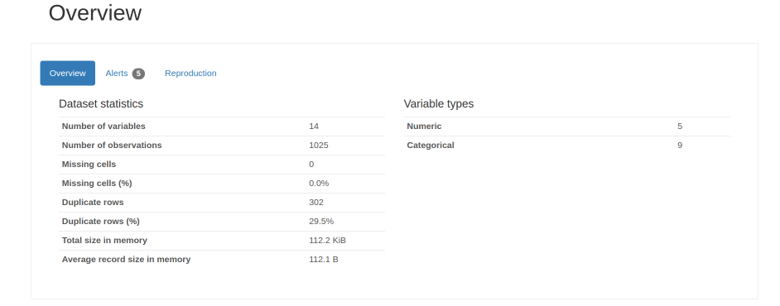
\includegraphics[width=0.8\linewidth]{TemplateTesi//immagini/tool1.png}
    \caption{Overview Generale fornita dall'applicativo}
    \label{fig:overviewapp}
\end{figure}
\begin{figure}
    \centering
    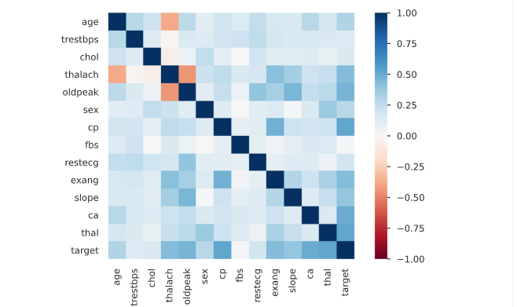
\includegraphics[width=0.7\linewidth]{TemplateTesi//immagini/tool2.png}
    \caption{HeatMap dei coefficienti di correlazione dell'applicativo}
    \label{fig:heatmapapp}
\end{figure}
\begin{figure}
    \centering
    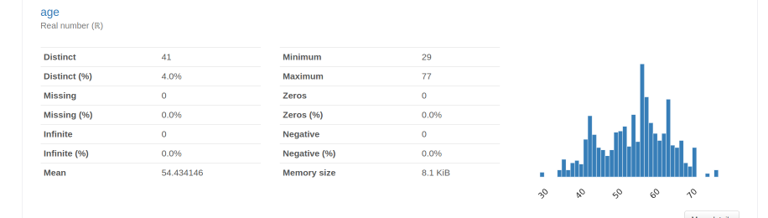
\includegraphics[width=0.7\linewidth]{TemplateTesi//immagini/tool3.png}
    \caption{Esempio di dati forniti dall'applicativo per ogni feature}
    \label{fig:datiapp}
\end{figure}
\begin{figure}
    \centering
    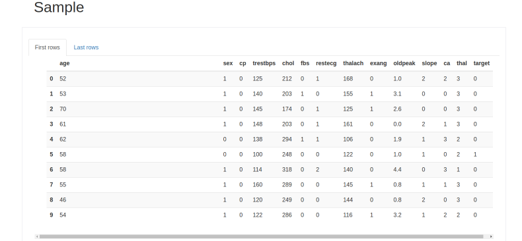
\includegraphics[width=0.7\linewidth]{TemplateTesi//immagini/tool4.png}
    \caption{Sample Mostrati dall'applicativo}
    \label{fig:sampleapp}
\end{figure}